\subsection[Elitism]{\label{identificadorReferenciaCruzada}
Elitism}

\ \ Elitism consists of archiving the best solutions generated during the search. Elitism in NSGA-II is evident in the general outline of the algorithm. The key phase here is the replacement of individuals in the old generation. Before the replacement phase individuals in the old generation are sorted according to their ?goodness? together with the newly generated o spring. This allows the best individuals of the older generation to be passed in the next generation. The mechanism can be seen in Figure 3. P(sub)t is the parents population and Q(sub)t is the o spring population at generation t. F1 are the best solutions from the combined populations (parents and
o spring). F2 are the second best solutions and so on.

\begin{figure}[h!]
\begin{center}
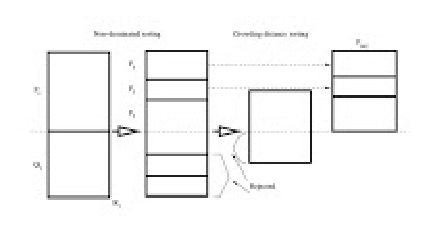
\includegraphics[width = 10cm] {./Graphics/Figure3.eps} 

\caption{Flow diagram that shows the way in which the NSGA-II elitism works.}
\end{center}
\end{figure}